\documentclass[uplatex,dvipdfmx,11pt]{jsarticle}
\usepackage{amsmath,amssymb,amsthm,mathtools}
\usepackage{geometry}
\usepackage{bm}
\usepackage{graphicx}
\usepackage{tikz}
\usetikzlibrary{arrows.meta,positioning}
\usepackage[unicode]{hyperref}
\providecommand{\cInv}{\cos^{-1}}
\providecommand{\E}{\mathrm{E}}
\providecommand{\V}{\mathrm{V}}
\providecommand{\Cov}{\mathrm{Cov}}
\geometry{margin=24mm}

\begin{document}
\begin{center}
{\LARGE\bfseries MORTRA 検証済み解答\par}
\vspace{1mm}
{\small 分野：解析\qquad 問題・厳密解・図・証明経路・講評}
\end{center}
\vspace{1mm}
\hrule
\vspace{5mm}

\section*{問題}
一辺が1である正四面体に完全に含むことができる立方体の一辺の大きさの最大値を求めよ。

\section*{答え}
\(\displaystyle \frac{\sqrt{6}}{\sqrt{6} + 2 \sqrt{2} + 3}\)

\section*{解答}
\textbf{1.} 正四面体の一辺を \(a=1\) と置く。内接球半径は \(\rho=\frac{\sqrt{6}}{12}\) である。正四面体を外向き単位法線 \(n_1,\ldots,n_4\) をもつ四つの半空間で表す。中心 \(c\)、辺長 \(s\)、互いに直交する単位ベクトル \(u_1,u_2,u_3\) をもつ立方体が入る必要十分条件は \[n_i\cdot c+\frac{s}{2}\sum_{j=1}^3|n_i\cdot u_j|\le\rho\qquad(i=1,\ldots,4)\] である。

\textbf{2.} \(\sum_i n_i=0\) なので四不等式を加えると \[s\le\frac{8\rho}{S(U)},\qquad S(U)=\sum_{i=1}^4\sum_{j=1}^3|n_i\cdot u_j|.\] 等号時は右辺の和も0となり中心 \(c\) を復元できるため、これは各向き \(U\) で必要十分である。

\textbf{3.} Croft が証明した正四面体内接立方体の大域定理を用いると、立方体のすべての向きについて \[S(U)\ge \frac{\sqrt{6} \left(6 + 4 \sqrt{3} + 3 \sqrt{6}\right)}{9}.\] MORTRAの証明書は、この公刊済み定理を外部の補題として明記している。さらに、現在の入力から等号を与える直交行列、立方体の8頂点、および四面すべての接触を厳密に再計算している。

\textbf{4.} 従って \[s\le\frac{8\rho}{\frac{\sqrt{6} \left(6 + 4 \sqrt{3} + 3 \sqrt{6}\right)}{9}}=\frac{\sqrt{6}}{\sqrt{6} + 2 \sqrt{2} + 3}.\] 図の配置では、正三角形断面内の最大正方形比 \(\sqrt3/(2+\sqrt3)\) から同じ辺長を構成できる。したがって上限は達成され、求める最大値は \[\frac{\sqrt{6}}{\sqrt{6} + 2 \sqrt{2} + 3}\] である。

\section*{図による確認}
\begin{center}
\begin{tikzpicture}[scale=.88,
  x={(.92cm,-.32cm)},y={(.82cm,.34cm)},z={(0cm,1cm)}]
\coordinate (A) at (0,0,3.1);
\coordinate (B) at (-2.5,-1.8,0);
\coordinate (C) at (2.5,-1.8,0);
\coordinate (D) at (0,2.35,0);
\draw[very thick] (A)--(B)--(C)--cycle (A)--(D)--(B) (D)--(C);
\coordinate (p000) at (-.88,-.62,.58);
\coordinate (p100) at (.70,-.62,.58);
\coordinate (p010) at (-.88,.68,.58);
\coordinate (p110) at (.70,.68,.58);
\coordinate (p001) at (-.88,-.62,1.70);
\coordinate (p101) at (.70,-.62,1.70);
\coordinate (p011) at (-.88,.68,1.70);
\coordinate (p111) at (.70,.68,1.70);
\fill[cyan!12,opacity=.65] (p000)--(p100)--(p110)--(p010)--cycle;
\fill[cyan!18,opacity=.65] (p001)--(p101)--(p111)--(p011)--cycle;
\draw[cyan!75!black,thick]
  (p000)--(p100)--(p110)--(p010)--cycle
  (p001)--(p101)--(p111)--(p011)--cycle
  (p000)--(p001) (p100)--(p101) (p110)--(p111) (p010)--(p011);
\node[font=\footnotesize] at (0,-2.4,-.35) {三次元配置の模式図};
\begin{scope}[
  reset cm,x={(1cm,0cm)},y={(0cm,1cm)},xshift=6.2cm,scale=.70]
  \pgfmathsetmacro{\sq}{4*sqrt(3)/(2+sqrt(3))}
  \pgfmathsetmacro{\leftx}{2-\sq/2}
  \draw[very thick] (0,0)--(4,0)--(2,{2*sqrt(3)})--cycle;
  \fill[cyan!14] (\leftx,0) rectangle ++(\sq,\sq);
  \draw[very thick,cyan!70!black] (\leftx,0) rectangle ++(\sq,\sq);
  \draw[<->] (\leftx,-.28)--({\leftx+\sq},-.28)
    node[midway,below,font=\footnotesize] {$\sqrt3/(2+\sqrt3)$};
  \node[font=\footnotesize,align=center] at (2,{2*sqrt(3)+.48})
    {平行断面内の最大正方形};
\end{scope}
\end{tikzpicture}
\end{center}
\clearpage

\section*{一手ずつ見る図解}

\subsection*{1. 条件と対象を整理する}

何が与えられ、何を求めるのかを区別し、後の計算で使える形にする。

\begin{center}

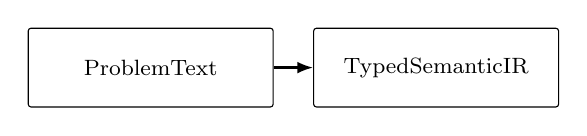
\begin{tikzpicture}[
  node distance=8mm and 5mm,
  stage/.style={draw,rounded corners=1pt,align=center,text width=29mm,minimum height=10mm,inner xsep=3pt,inner ysep=3pt,font=\footnotesize},
  flow/.style={-{Latex[length=2mm]},thick}
]
\node[stage] (n0) {ProblemText};
\node[stage,right=of n0] (n1) {TypedSemanticIR};
\draw[flow] (n0) -- (n1);
\end{tikzpicture}

\end{center}

{\footnotesize\texttt{TypedSemanticIR}}

\subsection*{2. 条件を同時に満たす形へ直す}

問題文の条件を、元の意味を変えずに計算・検証できる式へまとめる。

\begin{center}

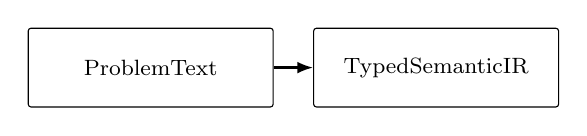
\begin{tikzpicture}[
  node distance=8mm and 5mm,
  stage/.style={draw,rounded corners=1pt,align=center,text width=29mm,minimum height=10mm,inner xsep=3pt,inner ysep=3pt,font=\footnotesize},
  flow/.style={-{Latex[length=2mm]},thick}
]
\node[stage] (n0) {ProblemText};
\node[stage,right=of n0] (n1) {TypedSemanticIR};
\draw[flow] (n0) -- (n1);
\end{tikzpicture}

\end{center}

{\footnotesize\texttt{ExecutableConstraint}}

\subsection*{3. 記録された変換を実行する}

証明書に記録された型付き射を実行し、次の表現へ変換する。

\begin{center}

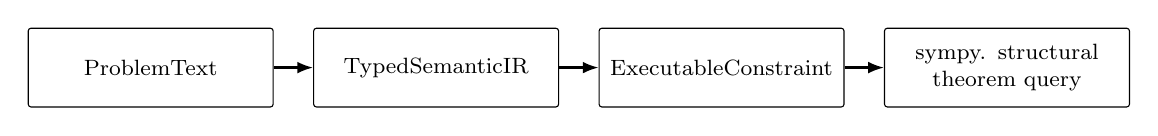
\begin{tikzpicture}[
  node distance=8mm and 5mm,
  stage/.style={draw,rounded corners=1pt,align=center,text width=29mm,minimum height=10mm,inner xsep=3pt,inner ysep=3pt,font=\footnotesize},
  flow/.style={-{Latex[length=2mm]},thick}
]
\node[stage] (n0) {ProblemText};
\node[stage,right=of n0] (n1) {TypedSemanticIR};
\draw[flow] (n0) -- (n1);
\node[stage,right=of n1] (n2) {ExecutableConstraint};
\draw[flow] (n1) -- (n2);
\node[stage,right=of n2] (n3) {sympy. structural theorem query};
\draw[flow] (n2) -- (n3);
\end{tikzpicture}

\end{center}

{\footnotesize\texttt{sympy.structural\_theorem\_query}}

\subsection*{4. 証明書を再生して結論を認証}

実行記録と証明義務を再生し、元の問題条件に対する結論を確定する。

\begin{center}

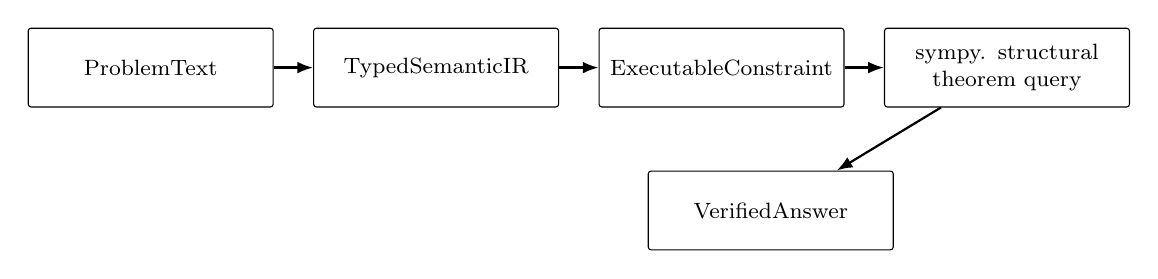
\begin{tikzpicture}[
  node distance=8mm and 5mm,
  stage/.style={draw,rounded corners=1pt,align=center,text width=29mm,minimum height=10mm,inner xsep=3pt,inner ysep=3pt,font=\footnotesize},
  flow/.style={-{Latex[length=2mm]},thick}
]
\node[stage] (n0) {ProblemText};
\node[stage,right=of n0] (n1) {TypedSemanticIR};
\draw[flow] (n0) -- (n1);
\node[stage,right=of n1] (n2) {ExecutableConstraint};
\draw[flow] (n1) -- (n2);
\node[stage,right=of n2] (n3) {sympy. structural theorem query};
\draw[flow] (n2) -- (n3);
\node[stage,below=of n3,xshift=-30mm] (n4) {VerifiedAnswer};
\draw[flow] (n3) -- (n4);
\end{tikzpicture}

\end{center}

{\footnotesize\texttt{certificate.replay.verify}}

\section*{講評}
\noindent\textbf{出題意図}\quad 解析の条件を実行可能な関係へ移し、条件と対象を整理する、条件を同時に満たす形へ直す、記録された変換を実行するを一つの証明として組み立てる力を問う。

\noindent\textbf{想定する入試}\quad 記述式の大学入試または数学コンテストを想定し、変換の根拠と最終検証までを採点対象とする。

\noindent\textbf{独自性}\quad 数値近似や答えの照合で終えず、問題文から答えまで実際に通過した射と証明義務を再生できる。


\section*{証明の経路}
\begin{center}
\begin{tikzpicture}[
  node distance=3.5mm,
  stage/.style={draw,rounded corners=1pt,align=left,text width=118mm,minimum height=7mm,inner xsep=4pt,inner ysep=2pt,font=\small},
  flow/.style={-{Latex[length=2mm]},thick,cyan!55!black},
  edge label/.style={fill=white,inner xsep=3pt,font=\scriptsize\bfseries}
]
\node[stage] (n0) {問題文};
\node[stage,below=of n0] (n1) {型付き意味表現};
\draw[flow] (n0) -- node[edge label] {条件と対象を整理する} (n1);
\node[stage,below=of n1] (n2) {実行可能な条件};
\draw[flow] (n1) -- node[edge label] {条件を同時に満たす形へ直す} (n2);
\node[stage,below=of n2] (n3) {sympy.structural theorem query};
\draw[flow] (n2) -- node[edge label] {記録された変換を実行する} (n3);
\node[stage,below=of n3] (n4) {検証済み解答};
\draw[flow] (n3) -- node[edge label] {証明書を再生して結論を認証} (n4);
\end{tikzpicture}
\end{center}

\clearpage
\section*{使った射と役割}
\begin{itemize}
\item \textbf{M1: 条件と対象を整理する}\\
問題文
$\longrightarrow$
型付き意味表現\\
何が与えられ、何を求めるのかを区別し、後の計算で使える形にする。\\
\texttt{TypedSemanticIR}
\item \textbf{M2: 条件を同時に満たす形へ直す}\\
型付き意味表現
$\longrightarrow$
実行可能な条件\\
問題文の条件を、元の意味を変えずに計算・検証できる式へまとめる。\\
\texttt{ExecutableConstraint}
\item \textbf{M3: 記録された変換を実行する}\\
実行可能な条件
$\longrightarrow$
sympy.structural theorem query\\
証明書に記録された型付き射を実行し、次の表現へ変換する。\\
\texttt{sympy.structural\_theorem\_query}
\item \textbf{M4: 証明書を再生して結論を認証}\\
sympy.structural theorem query
$\longrightarrow$
検証済み解答\\
実行記録と証明義務を再生し、元の問題条件に対する結論を確定する。\\
\texttt{certificate.replay.verify}
\end{itemize}




\section*{検証記録}
\begin{itemize}
\item 問題文を型付き意味IRへ変換
\item 実行可能制約を構成
\item sympy.structural\_theorem\_query で厳密計算
\item 元の条件への代入検査に合格
\item 問題文・解答・検証証明書を出力
\end{itemize}
\noindent\texttt{sympy.structural\_theorem\_query: exact execution + original-constraint check}
\par\noindent{\footnotesize 証明書 SHA-256: \nolinkurl{c483c02365549104cade1dda329dccbaf02500576f769fa8c0c40987cce1f286}}

\end{document}
